\section{Introduction}

Large Language Models (LLMs) have demonstrated remarkable performance when augmented with retrieval mechanisms. Traditional retrieval-augmented generation (RAG) primarily targets open-domain corpora, seeking to retrieve and integrate \emph{objective facts}~\citep{lewis2020retrieval,li2025search,chen2024benchmarking, han2024retrieval}. In contrast, \emph{memory retrieval} focuses on user-specific histories, preferences, and contextualized interactions, aiming to surface evidence tailored to \emph{a particular user at a specific moment}~\citep{zhong2024memorybank,jiang2025know,tan2025personabench,wu2024longmemeval,xu2025towards}, as illustrated in the top of Figure~\ref{fig:intro}. The design of memory fundamentally shapes the boundary of personalized LLMs~\citep{zhang2025survey}: it can remain a static external index passively queried, or evolve into a dynamic process of recollection, thereby endowing the system with a more human-like flow of memory~\citep{wu2025human,hatalis2023memory}. 
Just as humans sometimes recognize a familiar face instantly (i.e., an intuitive ``feeling of knowing'' without deliberate reasoning) and at other times reconstruct past experiences through slow chains of recollection, so too should memory retrieval move beyond static lookup. A personalized LLM needs to be flexible and alternate between fast recognition and gradual reconstruction, adapting to the demands of the interaction.

\begin{figure}[htbp]
\centering
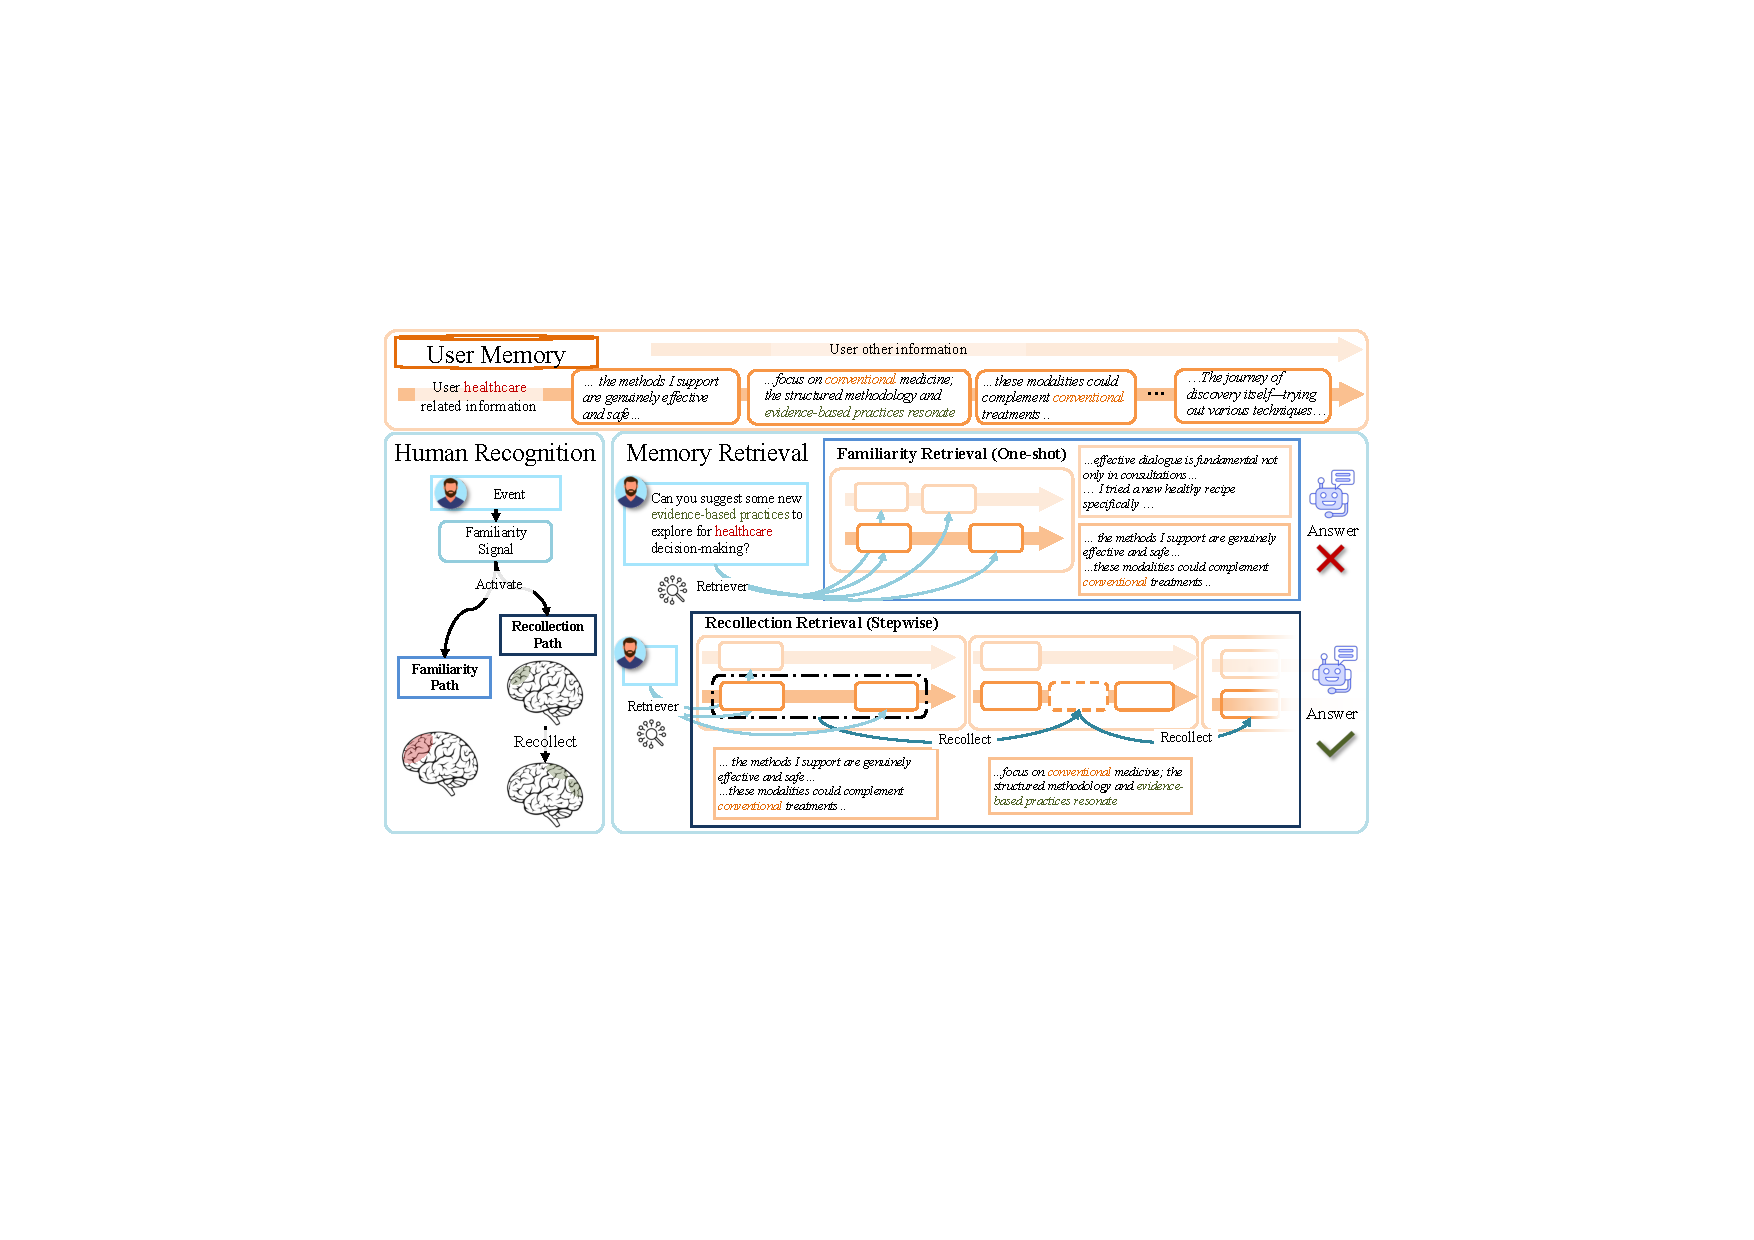
\includegraphics[width=0.95\linewidth]{chapter/figure/Intro.pdf}
\caption{Comparison between standard familiarity-based retrieval and recollection-based retrieval in user health narratives. And the brain figure motivated by~\citep{rugg2007event, yonelinas2024role}.}
\label{fig:intro}
\vspace{-10pt}
\end{figure}

Insights from cognitive science highlight the \emph{Recollection-Familiarity Dual-Process Theory}, as shown in Figure~\ref{fig:intro} left, which posits that human recognition and memory are driven by two complementary mechanisms~\citep{henson1999recollection, yonelinas2002effects, merkow2015human, bastin2019integrative, yonelinas2024role}. \emph{Familiarity} provides a rapid but coarse sense of ``knowing'', enabling efficient yet shallow judgments. \emph{Recollection}, in contrast, is triggered when familiarity proves insufficient, initiating a slower contextual reconstruction process that retrieves time, place, and source-specific details. Importantly, humans regulate these two processes via the familiarity signal: high confidence sustains reliance on familiarity, whereas decreasing familiarity and rising uncertainty prompt the shift to recollection~\citep{rugg2007event, yonelinas2024role}. Applied to user memory retrieval in personalized LLMs, this theory suggests that retrieval should not be conceived as a one-shot operation. Instead, it should function as a dual-process controller that adaptively alternates between fast recognition and slow recollection, guided by the system's sense of familiarity.


Current retrieval systems often reduce memory to a static set of vectors, relying on direct similarity search without mechanisms to evoke richer user recollections. Retrieval in memory-augmented LLMs can be understood along three dimensions: query reformulation~\citep{li2025hello, zhao2025memocue, chen2025llm, shen2024retrieval, salama2025meminsight}, index construction~\citep{zhong2024memorybank, pan2025secom, xu2025towards, tan2025prospect, xu2025mem, ong2024towards,chhikara2025mem0}, and retrieval strategy~\citep{xu2021beyond}. While existing work has advanced the first two, retrieval strategies remain dominated by embedding-based one-shot top-$K$ search~\citep{karpukhin2020dense, lei2023unsupervised, wang2020minilm, song2020mpnet, luo2024bge}, corresponding to the \emph{Familiarity} channel: fast yet shallow recall. 
% This overlooks the \emph{Recollection} path (i.e., stepwise, context-driven reconstruction) crucial for handling ambiguous queries, long-tail knowledge, or personalization. 
% Without progressive recollection and uncertainty-driven switching between familiarity and recollection, current systems either under-retrieve, missing deeper contextual cues, or over-retrieve, introducing irrelevant noise. 
\yy{
Two key limitations remain in current memory retrieval systems:  
\textbf{1) they overlook the \emph{Recollection} path}, failing to retrieve evidence chains for ambiguous queries, long-tail knowledge, or personalized reasoning;  
\textbf{2) they lack mechanisms for path switching between familiarity and recollection}, leading to either under-retrieval that misses deeper contextual cues or over-retrieval that introduces more retrieval latency.}
% \yc{this is our method not the reason}
As shown in Figure~\ref{fig:intro}, the \emph{Familiarity} path may retrieve only partial fragments (e.g., ``I support are genuinely effective and safe''), missing broader context and even introducing irrelevant noise (e.g., ``new healthy recipe''). By contrast, the \emph{Recollection} path expands iteratively and can introduce more \yy{comprehensive evidence} (e.g., ``focus on conventional medicine; and evidence-based practices resonate''). 
% \yc{-only?}
\yy{This gap underscores the need for a recollection retrieval path and adaptive switch mechanism to balance efficiency with reliable coverage.}

% \yc{it seems the limitations are not listed clear as 1,2,3? so, the limitations is 1. adaptive, 2. ?}
To address these limitations, we propose \textbf{RF-Mem} (\textbf{R}ecollection–\textbf{F}amiliarity \textbf{Mem}ory Retrieval), an uncertainty-guided dual-path retrieval framework. RF-Mem begins with a probe retrieval that produces an initial retrieval list and estimates its familiarity by computing the mean score and entropy in the list. When familiar, the system stays on the \emph{Familiarity} path, returning the top-$K$ candidates in a \textit{one-shot} manner with minimal overhead. Otherwise, RF-Mem activates the \emph{Recollection} path: the probe results are clustered by KMeans, each cluster centroid is combined with the original query through an $\alpha$-mixing strategy, and the resulting recollect-queries are expanded iteratively. At each round, new candidates are retrieved, clustered, and mixed to form updated queries, allowing the system to \textit{stepwise} reconstruct evidence chains. The process is explicitly bounded by beam width, fanout, and maximum rounds, ensuring controllable computation. In this way, RF-Mem preserves the efficiency of single-pass retrieval when familiarity is high, while adaptively engaging structured recollection under unfamiliar conditions, embedding chain-like reasoning directly into the retriever.

Our contributions are fourfold:  
(1) We ground the design of personalized memory retrieval in the Recollection–Familiarity dual-process theory, formulating retrieval as a coordination of Familiarity and Recollection paths.  
(2) We introduce familiarity uncertainty-driven selection for adaptive switching between Familiarity and Recollection.  
(3) We develop a recollection retrieval based on clustering and query–centroid mixing, achieving chain-like evidence reconstruction only in embedding space.  
% (4) RF-Mem relies on lightweight vector search and clustering, offering a low-latency implementation. 
\yy{(4) RF-Mem is lightweight, relying solely on vector search and small-scale clustering, achieving high accuracy and recall at near one-shot retrieval latency.}
% \yc{use declarative sentence, we provide a light/high efficient development/implementation} 
Extensive experiments on three personalized memory datasets show that RF-Mem consistently surpasses both one-shot top-$K$ retrieval and the full-context method with low latency. An adaptive study shows that RF-Mem complements and generalizes to index-building methods like MemoryBank~\citep{zhong2024memorybank}.
% Just as humans sometimes recognize a familiar face in an instant, which is a rapid ``feeling of knowing'' without deliberate reasoning, and at other times narrate life stories through a slow chain of recollections, where one summer scene evokes related people, places, and emotions, so too should memory retrieval transcend static lookup and flexibly alternate between fast recognition and slow reconstruction. 
% Current retrieval systems, however, largely reduce memory to a static set of vectors, without mechanisms to evoke or expand beyond direct similarity. To endow LLMs with a personalized capacity for ``recollection,'' retrieval should extend beyond static lookup and evolve into a dynamic process of evidence reconstruction.


% familiarity is insufficient, engaging a chain of contextual reconstruction that retrieves time, place, and source-specific details with higher diagnostic value but at greater cost. Crucially, humans regulate these two processes through familiarity signal: when familiarity confidence is high, recognition relies on familiarity; when familiarity decreases and uncertainty rises, recollection is invoked~\citep{rugg2007event, yonelinas2024role}. 
% Anchoring this to user memory retrieval, for personalized LLMs, this implies that retrieval should not be single-pass, but rather a dual-process controller that adaptively switches between fast recognition and slower recollection in response to familiarity with uncertainty. 

% Anchoring this to user memory retrieval, Figure~\ref{fig:intro} contrasts a standard familiarity pass that surfaces only salient fragments in a patient narrative (for instance, “alternative practices often lacked scientific evidence”) with a recollection pass that integrates temporally distributed details (for instance, prior beliefs, the need to gather patient history, and evolving behaviors), thereby yielding a more actionable and individualized summary for decision support. For personalized LLMs, this implies that retrieval should not be single-pass, but rather a dual-process controller that adaptively switches between fast recognition and deeper recollection in response to predictive uncertainty. 


% As illustrated in Figure~\ref{fig:intro}, familiarity recall may surface only a salient fragment (e.g., ``alternative practices lacked scientific evidence''), whereas recollection can rebuild temporally distributed details (e.g., patient history and evolving behaviors), yielding more diagnostic evidence. This gap highlights the need for retrieval policies that adaptively integrate familiarity and recollection, balancing efficiency with contextual coverage.

% Current retrieval systems, however, largely reduce memory to a static set of vectors, without mechanisms to evoke user memory beyond direct similarity. Retrieval in memory-augmented LLMs can be analyzed in three dimensions: the reformulation of the query~\citep{li2025hello, zhao2025memocue, chen2025llm, shen2024retrieval, salama2025meminsight}, the index building of the memory data~\citep{zhong2024memorybank, pan2025secom, xu2025towards, tan2025prospect, xu2025mem, ong2024towards,chhikara2025mem0, rasmussen2025zep}, and the retrieval strategy~\citep{xu2021beyond} that governs how memories are retrieved. Existing work has primarily advanced the first two—designing query reformulations and optimizing index structures, that while leaving the retrieval policy itself to rely on embedding models~\citep{karpukhin2020dense, lei2023unsupervised, wang2020minilm, song2020mpnet, luo2024bge} to perform a one-shot top-$k$ procedure. This bias corresponds to the \emph{Familiarity} channel, offering fast but shallow recall, and overlooks the chain-based contextual reconstruction characteristic of \emph{Recollection}, which is critical under ambiguous queries or sparse signals. 

% As a result, most retrieval modules of these methods fail to adapt to task difficulty or user demand, and thus lack progression and contextual rebuilding. Two key limitations arise from this gap. First, neglect the \emph{stepwise recollection} emphasized in dual-process theory: without progressive context reconstruction, retrieval remains shallow and struggles with complex queries, long-tail knowledge, and context-bound personalization. Second, the absence of an uncertainty-driven mechanism for switching between Familiarity and Recollection often leads to retrieval that is either insufficient which failing to capture deeper contextual cues, or noisy, introducing redundant or irrelevant evidence. As illustrated in Figure~\ref{fig:intro}, a familiarity pass surfaces only a salient fragment (e.g., “alternative practices lacked scientific evidence”), whereas recollection reconstructs temporally distributed details (e.g., the need to gather patient history and evolving behaviors), yielding more diagnostic evidence. This motivates a retrieval design that adaptively integrates familiarity and recollection, deciding when to fast familiarity recall and when to recollect by familiarity uncertainty signal to balance efficiency with coverage.

% o	现在的检索主要是什么检索？基于LLM的上下文检索，或者embedding检索。RAG的embedding检索是基于一个embedding模型来做topk检索。讲讲这一类方法的问题。
% o	量化隐空间的慢思考和llm生成的慢思考。讨论我们的逻辑性，我们更细粒度，更稳定。我们是确定性的方法，对比llm是不确定性的方法。
% o	补实验：全上下文输入+慢思考模型，对比我们的隐空间慢思考检索。提供evidence。我们高效稳定。
% o	有个性化的keywords。要讲这一类方法存在的问题，现有的dense检索无法结构式或者链式的框架的。引出我们的问题1和问题2。多加文献，一方面来自motivation，一方面来自现有工作的不足。
% 
% Despite rapid progress in memory-augmented LLM, existing approaches remain mismatched to this perspective. Most systems implement retrieval as a fixed top-$k$ similarity search, corresponding to the Familiarity channel, with no mechanism for chain-like recollection. This limitation leads to poor coverage for complex queries, long-tail knowledge, and context-sensitive personalization. Other methods attempt to mitigate this gap via LLM-based query expansion (e.g., interleaving retrieval and generation). While such extensions superficially resemble Recollection, they substantially increase latency and computational cost. Moreover, these methods place the burden of innovation on the generator, leaving retrieval itself a passive module without structure or adaptivity. As a result, current memory systems lack both the chain-based properties of recollection and the uncertainty-driven switching mechanism emphasized in dual-process theory. This motivates our research question: \emph{Can we design a retrieval strategy that dynamically and adaptively combines Familiarity and Recollection, enabling personalized LLMs to decide—based on uncertainty—when to stop at fast recall and when to enter deeper recollection, thereby achieving a balanced trade-off between efficiency and adaptivity?}


% To address these limitations, we propose \textbf{RF-Mem} (\textbf{R}ecollection–\textbf{F}amiliarity \textbf{Mem}ory Retrieval), an uncertainty-guided dual-path retrieval framework. RF-Mem begins with a probe search that produces an initial retrieval list and estimates its familiarity by computing the mean score and entropy in the list. When entropy is low or the mean score is high, the system remains in the Familiarity path, performing a one-shot top-$K$ retrieval at minimal cost. When entropy is high or the mean score is low, RF-Mem transitions to the Recollection path: the initial candidates are clustered via KMeans, class centers are combined with the original query through an $\alpha$-mixing strategy by the embedding model, and the resulting recollect-queries are used for iterative retrieval and clustering. This iterative process incrementally reconstructs evidence chains, closely emulating human recollection. The depth of iteration and number of candidates are explicitly constrained, ensuring controllable cost. In this way, RF-Mem transcends the superficiality of single-pass retrieval and embeds adaptive recollection directly into the retriever.

% This process incrementally reconstructs evidence chains, emulating human recollection. Iteration is governed by the depth and the number of required candidate constraints, ensuring controllable cost. In this way, RF-Mem avoids the superficial coverage of single-shot retrieval and embeds adaptive recollection into the retriever.



